\documentclass[Main]{subfiles}
\begin{document}

\textbf{Optimization of implemented client}


- Ordering of goals and goals conflicting - maybe look for goals with most walls around (such as safe goals)

- Use partial plan as guideline for Heuristics

- Better subgoal decomposition

- "Better" back tracking

- Re-order goals?

- Multi-agent: Conflict handling

The current implementation lacks solid conflict handling when solving multi-agent levels. To make up for this, we propose to enhance the system with the methods described in \cite{pellier2007unified}.

In this paper, an algorithm is described for solving multi agent problems where a set of interdependent agents need to collaborate to solve a common goal.
The algorithm uses methodologies from POP, HTN and a communication scheme between the agents to ensure the unified planning is consistent.

The algorithm works by initializing a POP with a set of open goals for the whole level to be completed. Next, the algorithm will assign a complex action to each of the agents to solve a goal.
Hereafter, the algorithm will start to refine the complex actions into primitive actions.
The agents take turn in refining one step in their complex actions into a primitive action, such that the resulting unified plan is consistent for all time steps, meaning that there is defined a primitive action for all agents for all time steps.

If a conflict arises in the plan, a threat is created which the agents will try to solve with. The agents will first try to find a complex action to resolve the threat and next to refine the complex action.
If refining a complex action fails and there is no way to solve the threat, the algorithm must backtrack to the beginning of the failing complex action, and either try another refinement or attempt to refine one of the other agents complex actions first.
If this other refinement also fails, the algorithm will have to backtrack further back to the refinement of another previous complex action.

During the planning process the agents communicate about threats, repairs, partial plan completions and refutations.
A repair is a suggestion on how to repair a given threat.
A partial plan completion is the event that an agent has achieved a plan for its goals successfully.
A refutation is a message from one agent to another where the sender detects a conflict with his current plan and another agents move and therefore refutes the other agents action.

An example of a threat can be that one agent is standing in the way of another agent, or that a box is in the way of an agent and help is needed to move it out of the way.
A suggestion for a repair for a given threat, can be that an offending agent moves away from given path.
A refutation can be that an agent 0 refutes agent 1's action because because agent 1 is moving to the same place as agent 0, and in this case a solution could be to tell agent 1 to wait until agent 0 has passed.

Obviously, this algorithm will need a way to decide which agent should go first. These decisions are important, because a wrong decision could lead to a plan which is much longer than the optimal solution.
To remedy this, a set of social laws could be taken into account each time the algorithm needs to decide which agent should have priority to go first.
One rule could for example be, that the agent who is closest to completing his current goal gets first priority, and another rule could be that an agent who is carrying a box has higher priority than agents not carrying boxes.

\begin{figure}[h!]
	\centering
	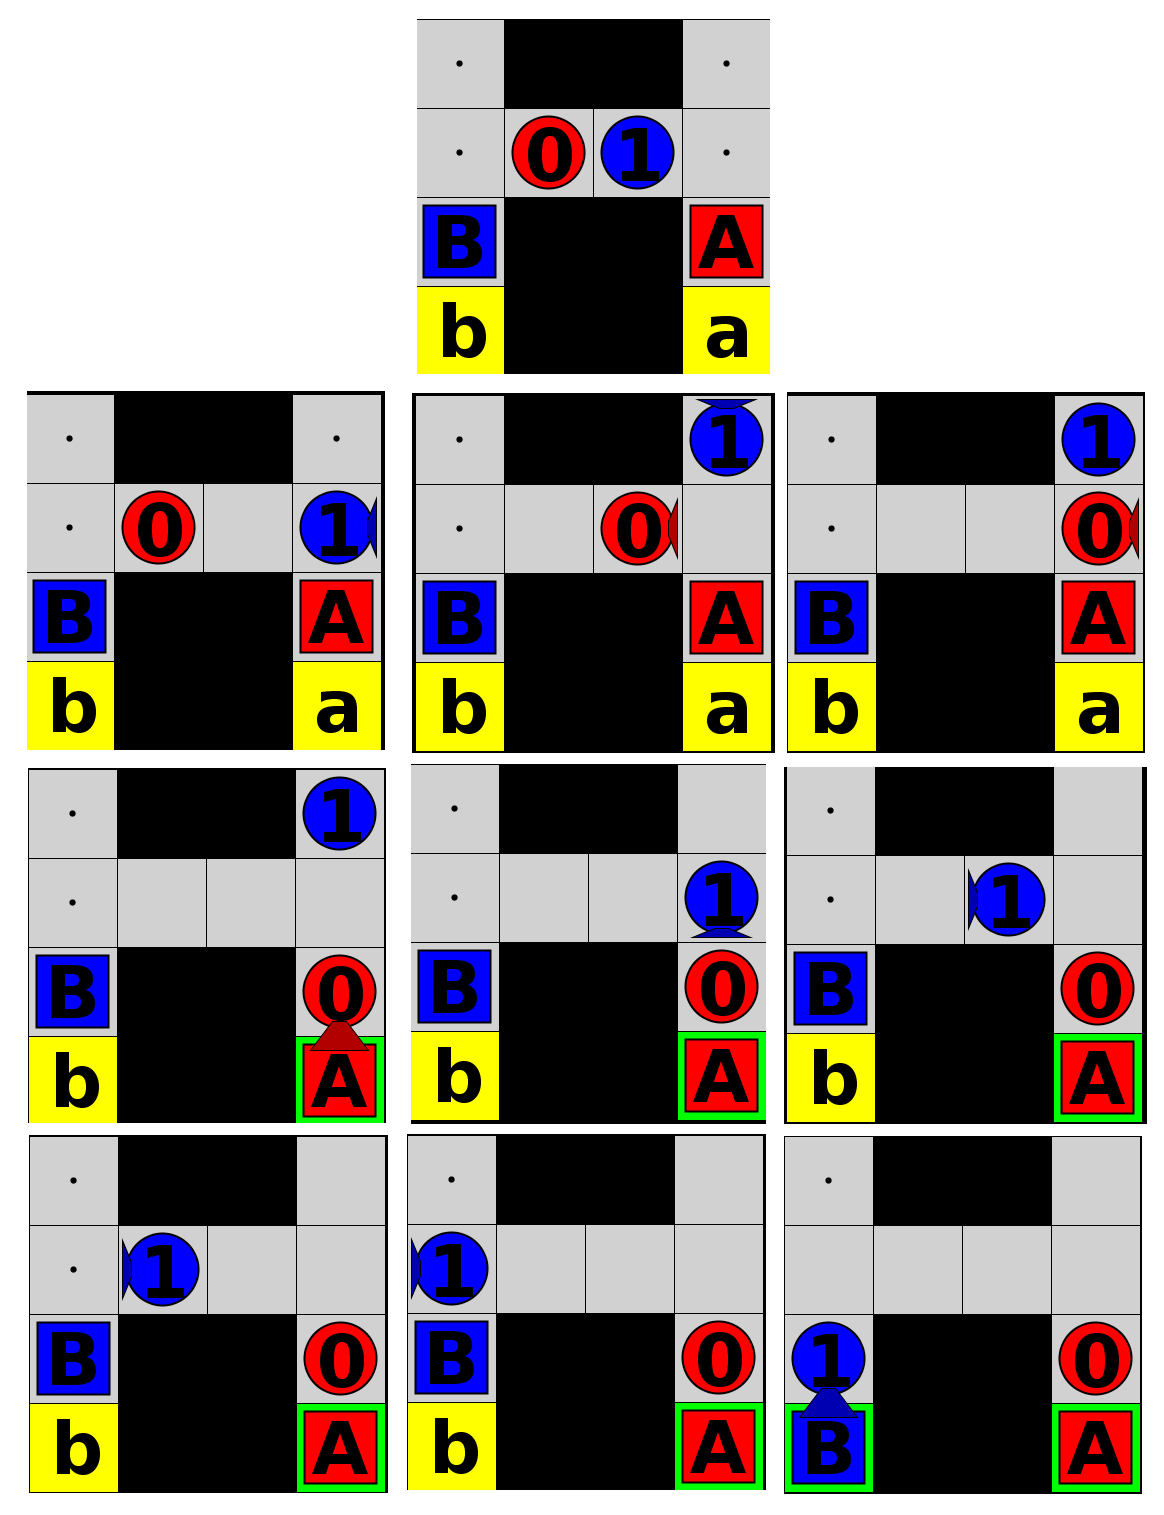
\includegraphics[width=0.3\textwidth]{plan_collab.png}
	\caption{Agent 0 needs to pass agent 1 in order to complete his goal, and vice versa}
	\label{fig:plan_collab}
\end{figure}

\begin{figure}[h!]
	\centering
	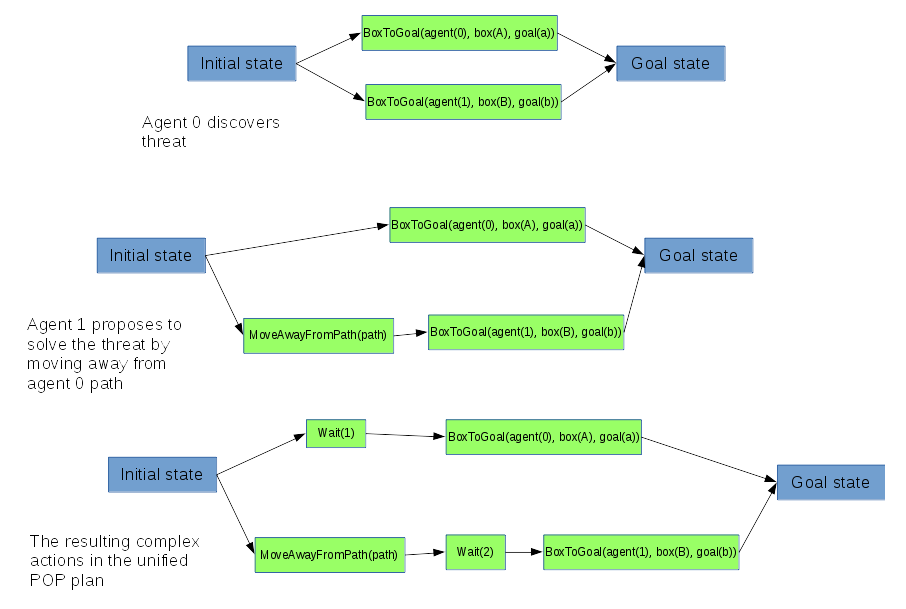
\includegraphics[width=0.5\textwidth]{unhtnpop.png}
	\caption{Example of a plan collaboration between agent 0 and 1 at complex action level}
	\label{fig:htn_collab}
\end{figure}

An example of the algorithm in action, is visualized in Figure \ref{fig:htn_collab} and \ref{fig:plan_collab}.

When agent 0 first tries to refine his complex action to complete goal 'a', he discovers that there is a conflict since agent 1 is standing in his way.
Agent 0 can thus report failure, and add a new threat to the set of unaccomplished threats for getting a clear path to his goal.

Next it is agent 1's turn to contribute to the plan. The agent picks the threat from the set of unaccomplished threats and assign a complex action to be completed before his own goal completion. Next the agent reports to all agents that he has found a repair to the unified plan.
Next, agent 0 will attempt to refine his plan again, but will get a refutation from agent 1 since he is in the process of moving out of the way.
Agent 1 will now suggest agent 0 to wait for one turn.
When agent 1 is out of the way, agent 0 can start refining his complex action to complete goal 'a'.
Since agent 1 has completed his complex action to move out of the way of agent 0, he will now attempt to refine his next complex action which is to complete goal 'b'.
However agent 0 will refute agent 1's action and ask him to wait, because agent 1 is moving into agent 0's current path.
This conflict will repeat until agent 0 is out of the way, and finally agent 1 can refine his complex action to solve goal 'b'.

\todo[inline]{Communication}

\todo[inline]{Auction of 'unsolvable' or expensive goals \cite{VanderKrogt2005}}
\todo[inline]{Cyclic dependencies}
\todo[inline]{\cite{Nguyen2001}}


\todo[inline]{Pruning algorithm to limit branching factor [http://en.wikipedia.org/wiki/Pruning\_(decision\_trees)]}
\todo[inline]{concurrency/parallel}

\end{document}
